% Template for ESA 6th ICATT manuscripts; to be used with:
%          spconf.sty  - LaTeX style file, and
%          IEEEbib.bst - IEEE bibliography style file.
% --------------------------------------------------------------------------
\documentclass{article}
\usepackage{spconf,amsmath,graphicx, url, listings}
\usepackage{courier, float}
\usepackage{caption}
\usepackage{subcaption}


\lstset{basicstyle=\footnotesize\ttfamily, float, language=MATLAB, breaklines=true}

% Example definitions.
% --------------------
\def\x{{\mathbf x}}
\def\L{{\cal L}}

% Title.
% ------
\title{Direct Trajectory Optimization of Upright Reusable Rocket Landing}
%
% Single address.
% ---------------
\name{Christopher Iliffe Sprague}
\address{}

\begin{document}

\maketitle

\begin{abstract}
    Recently within the aerospace industry, several demonstrations of successful soft, upright rocket landings have taken place; namely by SpaceX and Blue Origin. In this paper, such an application is examined through the scope of trajectory optimization and nonlinear programming. A general dynamical model of a rocket, equipped with a single thruster capable of gimbaling, is formulated. A direct method of discretizing state-time dynamics is applied to the dynamical model, from which a nonlinear program is developed. Using gradient based optimization, the nonlinear program representing the landing of a rocket is optimized with the objective of minimizing the rocket's propellant expenditure, while abiding to the constraints of landing \textit{softly} at the location of its target. It is shown that this paper's dynamical model and trajectory optimization method yield optimal propellant expenditures comparable with that of literature.
\end{abstract}
    
\keywords{Trajectory Optimization, Direct Methods}

\tableofcontents
\listoftables
\listoffigures
\lstlistoflistings


\section{Introduction}
The applications of trajectory optimization range from lunar landings to robotic locomotion. Through the developments of space exploration over the past few decades, new methods of spacecraft trajectory optimization of come to surface. Trajectory optimization problems have been tackled from a variety of perspectives, for example: optimal control \cite{Zhou2012}, machine learning \cite{DBLP:journals/corr/Sanchez-Sanchez16}, and convex programming \cite{Acikmese2007}. This paper takes the perspective of gradient based optimization.

\section{Trajectory Optimization}
Conventionally, in the case of a planetary lander, or in this case a rocket returning to Earth, trajectory optimization is performed using either direct or indirect methods. 
\subsection{Indirect Methods}
Indirect methods operate by first analytically constructing the necessary and sufficient conditions for optimality pertaining to the particular problem at hand, then secondly discretizing these conditions to formulate a constrained parameter optimization problem. Most often in the case of a planetary lander or the like, these necessary conditions are derived from Pontryagin's minimum principle \cite{Grabowski2009}. This principle states that, at every moment in time the dynamical system's control should be chosen to maximize the Hamiltonian of the system. The reader is advised to consult \cite{VonStryk1992} for my information about this method. 
\subsection{Direct Methods}
Direct methods operate by discretizing the trajectory optimization problem directly, in order to formulate a constrained parameter optimization problem. Direct transcription methods, in general, have several advantages over indirect transcription methods. The necessity to analytically determine initial costate variables is circumvented, and the optimization problem size is reduced by a factor of two. One of the most significant merits is that, one does not need to specify the structure of the problem, a priori. In general, direct transcription methods are very robust and are able to converge to optimal solutions from poor initial guesses.

\subsection{Problem Description}
For a general dynamical system, the problem of trajectory optimization is formulated as
\begin{equation*}
\begin{aligned}
& \underset{\mathbf{u}(t)}{\text{minimize}}
& & \phi(t_s,t_f,\mathbf{x_s},\mathbf{x_f}) + \int^{t_f}_{t_s} \mathcal{L}(\mathbf{x}(t),\mathbf{u}(t), t)dt\\
& \text{subject to}
& & \dot{\mathbf{x}} = \mathbf{a}(\mathbf{x},t) + \mathbf{u}(t)~\text{dynamic constraints}\\
&&& \mathcal{G}(t_s,t_f,\mathbf{x}_s,\mathbf{x}_f)\leq0 ~ \text{boundary conditions} \\
&&& \mathbf{u} \in \mathcal{U}(\mathbf{x},t) ~ \text{propulsion constraints}
\end{aligned}
\end{equation*}
Essentially, this formal formulation asks for the control at every moment in time $\mathbf{u}(t)$ in order to minimize the initial and terminal costs $\phi(t_s,t_f,\mathbf{x_s},\mathbf{x_f})$ and the path costs $\int^{t_f}_{t_s} \mathcal{L}(\mathbf{x}(t),\mathbf{u}(t), t)dt$, all while abiding to dynamic constraints and boundary constraints, which are all dictated by the state of the dynamical system $\mathbf{x}(t)$. For the case of a rocket landing, it is quite obvious that the boundary constraints would mandate that the rocket's final state $\mathbf{x}(t_f)$ be equal to the rocket's target state, which is chosen beforehand. The rocket's dynamic constraints are not as intuitive, and are derived from the way in which the system is discretized.

\subsection{System Description}
Following the common notation of optimal control, the trajectory of dynamical system can be formulated as a system of time-varying variables.
$$
\mathbf{z} = 
\begin{bmatrix}
\mathbf{x}(t) \\
\mathbf{u}(t)
\end{bmatrix}
$$
consisting of the system's \textit{state variables} $\mathbf{x}(t)$ and the \textit{control variables} $\mathbf{u}(t)$. Herein, vectors will be typeset in bold.

\subsubsection{State Variables}
The way in which the dynamical system evolves over time is described by the system dynamics. These dynamics, for the scope of this paper's discussion, are described by a system of ordinary differential equations, more commonly known as \textit{state equations}. The state equations, in their generic form, are written as
$$
\dot{\mathbf{x}} = \frac{d\mathbf{x}}{dt} = \mathbf{f}(\mathbf{x}(t),\mathbf{u}(t),t)
$$
Note that this description, in its generic form described a non-autonomous system, hence the right hand side's explicit dependence on time $t$. In the case of many aerospace applications, the system of ordinary differential equations governing its dynamics does not explicitly depend on time. For example, in the case of a spacecraft on an interplanetary trajectory, its dynamics do not depend on time, but rather the inverse square of its distance relative to surrounding celestial bodies.

\subsubsection{Boundary Conditions}
In the problem of trajectory optimization, two conditions must be strictly satisfied. That is, that the system's initial dynamic variables
$$
\mathbf{\psi}_0 = \mathbf{\psi}(\mathbf{x}(t_0),\mathbf{u}(t_0),t_0)
$$
at the initial time $t_0$, and the system's terminal dynamics variables,
$$
\mathbf{\psi}_f = \mathbf{\psi}(\mathbf{x}(t_f),\mathbf{u}(t_f),t_f)
$$
at the terminal time $t_f$ define the \textit{boundary conditions} of the trajectory optimization problem.

\subsubsection{Path Constraints}
In many dynamical systems, the problem of trajectory optimization leads itself to path constraints. These path constraints can range from obstacle avoidance in quad-copters to trajectory energy in spacecraft Lagrange point insertions. These path constraints can be formally stated as 
$$
\mathbf{g}(\mathbf{x}(t),\mathbf{u}(t),t) = 0
$$
Note, that this generic description of a trajectory optimization problem's path constraints forms a strong analogue to equality constraints in design optimization.

\subsubsection{System Bounds}
Of course, for many reasons it is necessary to bound a trajectory optimization problem, including, but not limited to: hardware constraints and simulation constraints. For example, one would bound the angular velocity of their fictional spacecraft so that it is not spinning into eternity. Additionally, one may want to place rectangular bounds on the environment of their spacecraft's simulation, for example: a spacecraft's position should be within the solar system. Aside from state constraints, there are also control constraints. In the case of the reusable rocket being examined in this paper, these constraints would be magnitude and direction of the rocket's thrust. The bounding on the system's state is formulated as
$$
\mathbf{x}_l \leq \mathbf{x}(t) \leq \mathbf{x}_u
$$
, and on the system's controls as 
$$
\mathbf{u}_l \leq \mathbf{u}(t) \leq \mathbf{u}_u
$$.

\subsubsection{Path Cost}
The whole point of trajectory optimization is select a control policy $\mathbf{u}(t)$ to minimize or maximize some measure of performance. In some cases, this measure of performance might be the time to travel from a starting location to an ending location in a dynamical system such as a quad copter. In the case of the rocket landing problem being investigated in this paper, the measure of performance is, of course, propellant expenditure. That is, the goal of the trajectory optimization process is to softly land the rocket at its target, while utilizing as little fuel as possible. For a general dynamical system, the path cost or objective function is defined as
$$
J = \phi(\mathbf{x}(t_0),\mathbf{x}(t_f),t_0,t_f)
$$
In the case of a landing that reduces fuel usage, otherwise know as a mass optimal landing, the final mass will be used explicitly to determine the measure of performance.

\subsection{Direct Transcription}
In direct transcription methods, the continuous state $\mathbf{x}(t)$ and control $\mathbf{u}(t)$ are discretized into a finite dimensional description. Through this technique, the original optimal control problem is transformed into a nonlinear programming problem (NLP). For the sake of intuition, transforming the nonlinear programming problem back to an optimal control problem would be akin to having an infinite quantity of states, controls, and constraints.

\subsubsection{Grid}
The first step in transforming a continuous optimal control problem into a finite dimension nonlinear programming problem is to define the resolution of the discretization $n$, or the number of nodes. Including the statement of the dynamical system's simulation starting time $t_I$ and final time $t_F$. From these statements, one can formulate the time grid
$$
[t_1,t_2.,\dots,t_n]
$$,
where one should note that $t_I = t_1$ and $t_F = t_n$, which form part of the system's boundary conditions. Intuitively, it is followed that the states are discretized as 
$$
\mathbf{x}_i = \mathbf{x}(t_i)
$$
and the controls as
$$
\mathbf{u}_i = \mathbf{u}(t_i)
$$

\subsubsection{Defects}
Once the system's original optimal control description has been transcribed through direct transcription, the values of the system's states $\mathbf{x}_i$ and controls $\mathbf{u}_i$ are represented by a (possibly) large set of NLP variables. The aforementioned bounds on both the system's state and control are simply instantiated at each node $n$ in the discretization. Perhaps the most crucial part of this direct trajectory optimization process is enforcing the system's inherent dynamics at each node. That is, an analytical quadrature procedure is used to compare the system's states at collocated nodes, in order to asses the validity of the optimizer's placement of each of the system's states. The schematic of this process can be seen in Figure \ref{fig:trajopt}.

\begin{figure}
    \centering
    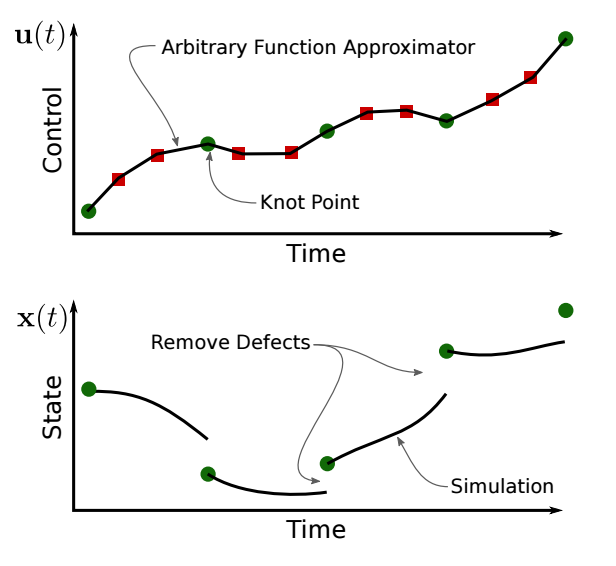
\includegraphics[width=0.48\textwidth]{pics/trajopt.png}
    \caption{Direction Transcription Schematic}
    \label{fig:trajopt}
    \cite{Nagy2001}
\end{figure}

\subsubsection{Nonlinear Programming Variables}
As previously noted, under the direct transcription process, in which the system's continuous state and control descriptions are transformed to a finite dimensional parameter constrained problem, a single NLP \textit{decision} vector is dealt with. This decision vector is formulated as
$$
\mathbf{z} =
\begin{bmatrix}
\mathbf{x}_0 \\
\mathbf{u}_0 \\
\mathbf{x}_1 \\
\mathbf{u}_1 \\
\vdots \\
\mathbf{x}_n \\
\mathbf{u}_n \\
t_0 \\
t_f 
\end{bmatrix}
$$,
where $t_0$ and $t_f$ are regarded as auxiliary variables. The auxiliary variables, in this case the time grid boundaries, determine the behaviour of the optimizer's manipulation of the state and control variables, through the time step size passed to the analytical quadrature method.

\subsection{Trapezoidal Transcription}
In order to compute the defects at each node in the grid space, a method to analytically propagate the system's dynamics is used. In this paper, herein the method of trapezoidal quadrature will be used. Within the grid space, at node $n$, the defect is defined as 
$$
\mathbf{\zeta}_n = \mathbf{x}_n - \mathbf{x}_{n-1} - \frac{h_n}{2}(\mathbf{f}_n + \mathbf{f}_{n-1})
$$.
Note that $h_n$ is the collocation step size, defined by
$$
h_n = t_n - t_{n-1}
$$,
and $\mathbf{f}_n$ is described by the system's equations of motion at node $n$ as
$$
\mathbf{f}_n = \mathbf{f}(\mathbf{x}(t_n),\mathbf{u}(t_n),t_n)
$$.
The resulting characterization of the defect forms the equality constraints of the dynamical system's trajectory optimization problem. If these equality constraints are satisfied at each node, then the dynamics of the optimized trajectory will be feasible according to trapezoidal quadrature.

\section{Rocket}
In order to optimize the trajectory of a rocket, it is first necessary to construct a dynamical model, which accurately describes a rocket's dynamics.
\subsection{Control}
It is appropriate to begin with defining the possible controls which the optimizer can take. In the case of a rocket, the main control is its thruster. While many thruster configurations exist for rockets, a common one to assume is a single thruster situated about the rocket's tail end, capable of gimbaling. With this configuration, in the reference frame of a rocket's body, the resulting control vector is formulated as $$ \mathbf{u_b} = \hat{\gamma}\Gamma $$, where $\hat{\gamma}$ is the direction of the thrust in the body's frame and $\Gamma$ is the magnitude of the thrust. The controls at any moment in time are defined as the thrust magnitude $\Gamma$, inclination angle $\eta$, and azimuth angle $\zeta$, describing the thrust vector in the body frame as $$ \mathbf{u_b} = \left[
\begin{array}{c}
 \Gamma  \sin (\zeta ) \cos (\eta ) \\
 \Gamma  \sin (\zeta ) \sin (\eta ) \\
 \Gamma  \cos (\zeta ) \\
\end{array}
\right] $$
This leads to the definition of the control vector
$$
\mathbf{A} = \left[
\begin{array}{c}
\Gamma \\
\eta \\
\zeta \\
\end{array}
\right]
$$

\subsection{Rigid Body}
It is sufficient to model the rocket as a cylinder, where the length of the rocket is $l$ and the radius of the rocket is $r$. 
\subsubsection{Orientation}
Firstly, it is necessary to establish some coordinate conventions. Firstly, the primary inertial reference frame is defined as a stationary reference frame, from which a body (i.e. the rocket) will be measured in reference to. The $Z$ axis is defined as being directed upward, out of the ground, towards the sky. The $X$ and $Y$ axes are arbitrarily directed, completing the triad forming the right handed coordinate system. 

The rocket's $z$ axis is taken to be directed from the rocket's tail to its nose, centered about its center of mass (i.e. halfway along the rocket's length for this discussion). Again, as with the inertial coordinate system, the rocket's $x$ and $y$ axes are arbitrarily defined to complete the triad, forming the right handed coordinate system. With these conventions, rotations about the rocket's $z$ axis is known as rolling, and rotations about the $x$ and $y$ axes describe pitching and yawing (somewhat arbitrarily since the rocket is axisymmetric).

The rocket's orientation in space with respect to the inertial frame of the simulation is robustly described using quaternions, rather than Euler angles, which often become vexatious due to their inherent propensity to encounter singularities. Taking the body's $z$ axis to be along its axial direction, positively away from the thruster's location, and the $x$ and $y$ axes to be arbitrarily directed orthogonally to the $z$ axis, completing the right-handed triad, the quaternion can be formulated as 
$$ \mathbf{q} = \left[
\begin{array}{c}
q_r \\
q_i \\
q_j \\
q_k \\
\end{array}
\right] $$
, where $\mathbf{q} = \left(1~0~0~0\right)^T$ describes the body's orientation to be in alignment with the inertial frame. Note that, as part of the NLP constraints, $q_r^2=q_i^2+q_j^2+q_k^2$. The resulting rotation matrix, describing the unit vectors of the body's axes, is computed as 
\begin{multline*}
\mathbf{R} = \\
\left[
\begin{array}{ccc}
 -2 q_j^2-2 q_k^2+1 & 2 \left(q_i q_j-q_k q_r\right) & 2 \left(q_i q_k+q_j
   q_r\right) \\
 2 \left(q_i q_j+q_k q_r\right) & -2 q_i^2-2 q_k^2+1 & 2 \left(q_j q_k-q_i
   q_r\right) \\
 2 \left(q_i q_k-q_j q_r\right) & 2 \left(q_i q_r+q_j q_k\right) & -2 q_i^2-2
   q_j^2+1 \\
\end{array}
\right]
\end{multline*}.
This rotation matrix allows vectors, originally described in the body's frame, to be represented in the inertial frame.
\subsubsection{Inertia}
Modelling the rocket as a cylinder with length $l$ and radius $r$, the three-dimensional inertia tensor can be formulated as 
$$
\mathbf{I} = \left[
\begin{array}{ccc}
 \frac{m}{12}  \left(3r^2+l^2\right) & 0 & 0 \\
 0 & \frac{m}{12}  \left(3r^2+l^2\right) & 0 \\
 0 & 0 & \frac{mr^2}{2} \\
\end{array}
\right]
$$.
which is used in the computation of the rocket's angular acceleration.
\subsection{Dynamics}\label{dynamics}
\subsubsection{Control}
Having constructed the robust quaternion based rotation matrix, the translational force due to the rocket's control vector in its local frame $\mathbf{u_b}$ can be described in the global inertial frame by premultiplying it by the aforementioned rotation matrix as follows
$$
\mathbf{u} = \mathbf{R}\cdot \mathbf{u_b}
$$.
Assuming the thruster's location in the rocket's coordinate system is $\mathbf{r_u}=\left(0~0~-l/2\right)^T$, the moment imparted by the control is
$$
\mathbf{\tau} = \left[
\begin{array}{c}
 -\frac{6 \Gamma  l \sin (\zeta ) \sin (\eta )}{l^2 m+m w^2} \\
 \frac{6 \Gamma  l \sin (\zeta ) \cos (\eta )}{l^2 m+m w^2} \\
 0 \\
\end{array}
\right]
$$

\subsubsection{Acceleration}
Having developed the model of the physical influences particular to the rocket environment, the full equation of translational motion is shown as 
$$
\frac{d^2\mathbf{p}}{dt^2} = \mathbf{g} + \frac{\mathbf{u}}{m}
$$
, where $\mathbf{p}$ is the position of the rocket, $\mathbf{g}=\left(0~0~-9.807\right)^T$ is the acceleration due to gravity, and $m$ is the mass of the rocket governed by
$$
\frac{dm}{dt} = -\frac{\Gamma}{\text{Isp}\cdot g}
$$,
where $\text{Isp}\approx 311~s$ is the specific impulse of the rocket's propulsion system. The angular acceleration of the rocket is as follows
$$
\frac{d\mathbf{\omega}}{dt} = \mathbf{\tau}\cdot \mathbf{I}^{-1}
$$,
where $\mathbf{\omega}$ is the rocket's angular velocity, from which the time rate of change of the quaternions, describing the rocket's orientation, can be computed through quaternion multiplication as follows
$$
\frac{d\mathbf{q}}{dt} = \frac{1}{2}
\left[
\begin{array}{c}
 0 \\
\mathbf{\omega} \\
\end{array}
\right] \otimes \mathbf{q}
$$
\subsection{State}
The state of the dynamical system, particular to the rocket, can be formalized as follows
$$
\mathbf{S} =
\left[
\begin{array}{cccc}
\mathbf{p}\\
\mathbf{v}\\
\mathbf{q}\\
\mathbf{\omega}\\
m\\
\end{array}\right]
=\left[
\begin{array}{cccccccccccccc}
x\\y\\z\\v_x\\v_y\\v_z\\q_r\\q_i\\q_j\\q_k\\
\omega_x \\ \omega_y \\ \omega_z \\ m
\end{array}\right]
$$ with a dimensionality of fourteen.

\section{Results}
Herein, in the analysis of this paper, the rocket's state is initialized as
$$
\mathbf{x}=[100,100,100,5,5,-5,1,0,0,0,0,0,0,10000]^T
$$
and the target's state is initialized as
$$
\mathbf{x}=[0,0,0,0,0,0,1,0,0,0,0,0,0,\text{None}]^T
$$.
Hence, the rocket has a mass of 10000 kilograms.
Note that the rocket is not given any target for its mass, as this is the metric to be optimized. The lower bound of the rocket's state is initialized as 
\begin{multline*}
\mathbf{LB}_\mathbf{x} = [-1000,-1000,0,-100,-100,-100,\\0,0,0,0,-100,-100,-100,0]^T
\end{multline*}
and the upper bound is initialized as
\begin{multline*}
\mathbf{UB}_\mathbf{x} = [1000,1000,1000,100,100,100,\\1,1,1,1,100,100,100,10000]^T
\end{multline*}.
In addition to the rocket's state, bounds are also placed on the rocket's controls. The control's lower bound is defined as
$$
\mathbf{LB}_\mathbf{u} = [0,0,0]^T
$$
and upper bound as
$$
\mathbf{UB}_\mathbf{u} = [44000,\pi,2\pi]^T
$$
Using the sequential quadratic programming algorithm, with five grid nodes $n=5$, a final mass of $m_f = 9863.16~kg$ is achieved, as shown Figure \ref{fig:conv5}. With ten grid nodes $n=10$, a final mass of $m_f=9902.53~kg$ is achieved, with a convergence seen in Figure \ref{fig:conv10}. Thus, as one can see, the accuracy of both the dynamical model and optimization method are confirmed, and more accurate results will be obtained with increasing nodes. The physical characterizations of the system's state and control for $n=5$, $n=10$, $n=15$, and $n=25$ nodes are seen in Figure \ref{fig:5nt}, \ref{fig:10nt}, \ref{fig:15nt}, \ref{fig:25nt}, respectively. The final masses achieved through this trajectory optimization process, among all node amounts, compare to that of an analogous example with equivalent metrics, using the indirect method, implemented in the documentation of the European Space Agency's open-source optimizer, PyGMO \cite{Izzo2012}. It should be noted, however, that increasing the number of nodes beyond $n=25$ proved to be incessant; even with parallel CPU core usage, computations were rather long winded do to sheer number of variables in the NLP problem.

\section{Conclusions}
This paper demonstrated a feasible trajectory optimization methodology to replicate the \textit{soft}, upright landing of a rocket, as first demonstrated by SpaceX and Blue Origin. Future improvements will include the migration to a low-level language, such as C++, to save on computational expenses. Additionally, different methods of transcription will be added to the current software library. And lastly, the software library will abstract itself to more general usage for such applications as interplanetary spacecraft trajectory optimization and quad-copters.

\begin{figure}
\includegraphics[width=0.5\textwidth]{pics/traj5nconv.eps} 
\caption{Convergence with 5 Nodes}\label{fig:conv5}
\end{figure}

\begin{figure}
\includegraphics[width=0.5\textwidth]{pics/traj10nconv.eps}
\caption{Convergence with 10 Nodes}\label{fig:conv10}
\end{figure}

\onecolumn
\begin{figure}
\includegraphics[width=1\textwidth]{pics/traj5n.eps}
\caption{Trajectory with 5 Nodes}\label{fig:5nt}
\end{figure}

\begin{figure}
\includegraphics[width=1\textwidth]{pics/traj10n.eps}
\caption{Trajectory with 10 Nodes}\label{fig:10nt}
\end{figure}

\begin{figure}
\includegraphics[width=1\textwidth]{pics/traj15n.eps}
\caption{Trajectory with 15 Nodes}\label{fig:15nt}
\end{figure}

\begin{figure}
\includegraphics[width=1\textwidth]{pics/traj25n.eps}
\caption{Trajectory with 25 Nodes}\label{fig:25nt}
\end{figure}

\twocolumn
\bibliographystyle{ieeetr}
\bibliography{refs.bib}

\section{Source Code}
\lstinputlisting[caption=Rocket Class - Matlab]{code/Rocket.m}
\lstinputlisting[language=python, caption=Rocket Class - Python]{code/Rocket.py}


\end{document}